\documentclass{beamer}
\usepackage[utf8]{inputenc}
\usepackage{graphicx}
\usepackage{amsmath, amssymb}
\usetheme{Madrid}
\usecolortheme{seahorse}
\title{Structural Loading on Appendages}
\subtitle{Understanding Lift, Bending, and Torsion in Natural Flyers}
\author{}
\date{}

\begin{document}

\frame{\titlepage}

\begin{frame}{Motivation}
\begin{itemize}
    \item Understand how nature handles aerodynamic forces
    \item Design better flying machines
    \item Predict and prevent structural failures
\end{itemize}
\end{frame}

\begin{frame}{Propulsive Appendages in Nature}
\begin{itemize}
    \item Fish fins, bird wings, insect wings
    \item Provide thrust and control
    \item Need to balance strength and flexibility
\end{itemize}

\vspace{0.5cm}
\begin{columns}
    \column{0.33\textwidth}
    \centering
    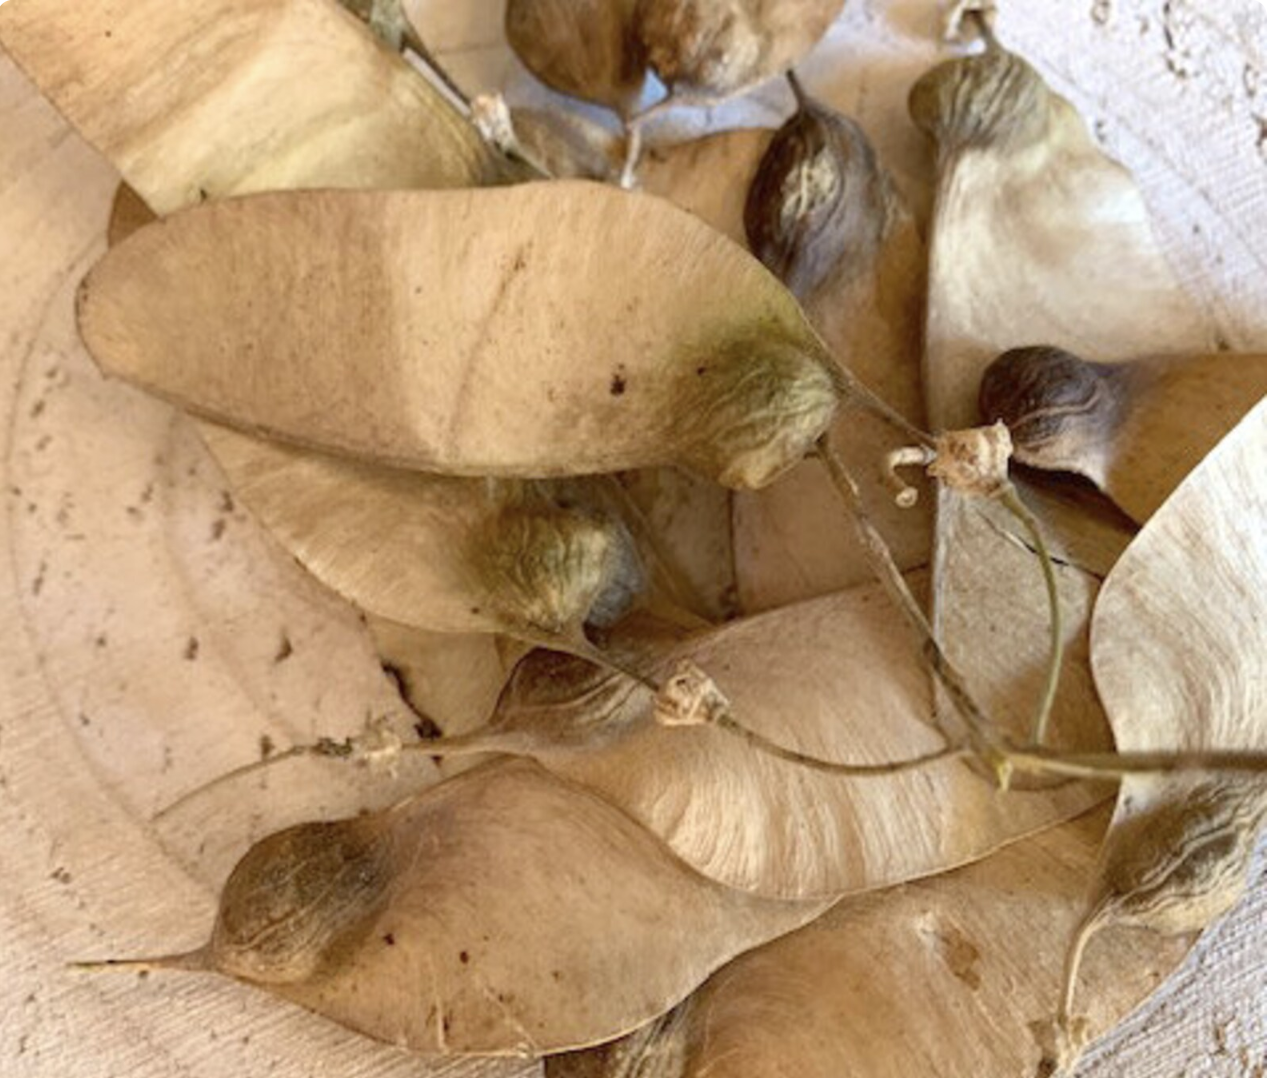
\includegraphics[width=\linewidth]{samara.png}
    
    \column{0.33\textwidth}
    \centering
    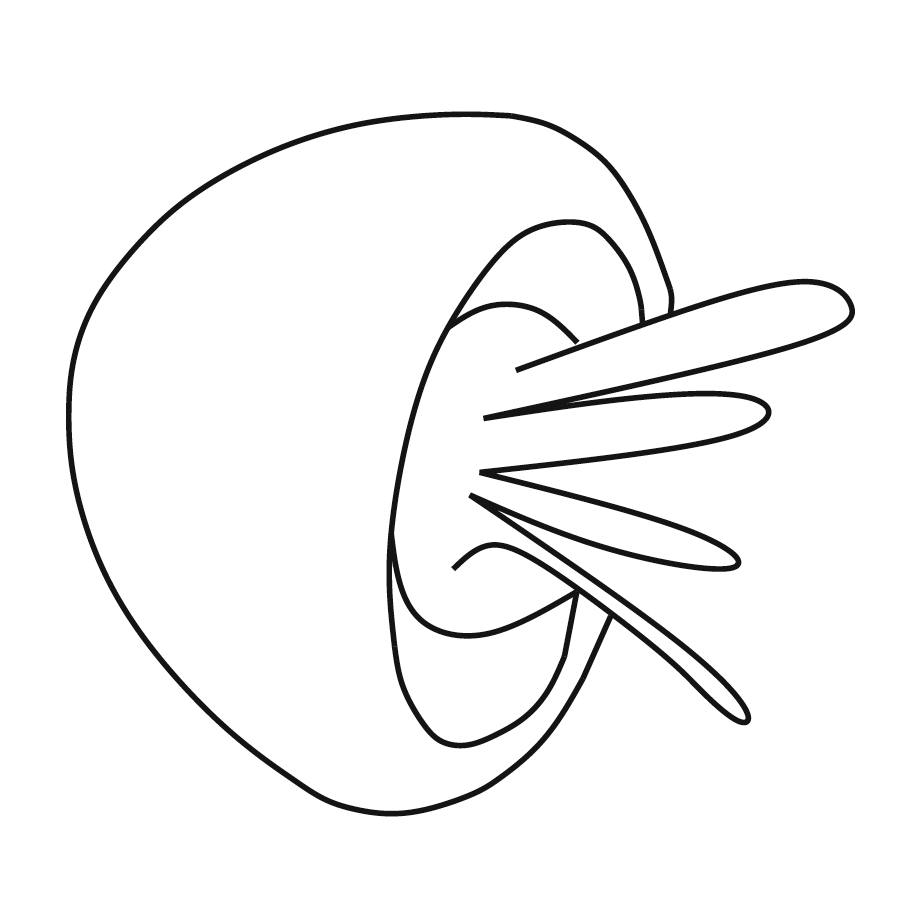
\includegraphics[width=\linewidth]{jelly.png}
    
    \column{0.33\textwidth}
    \centering
    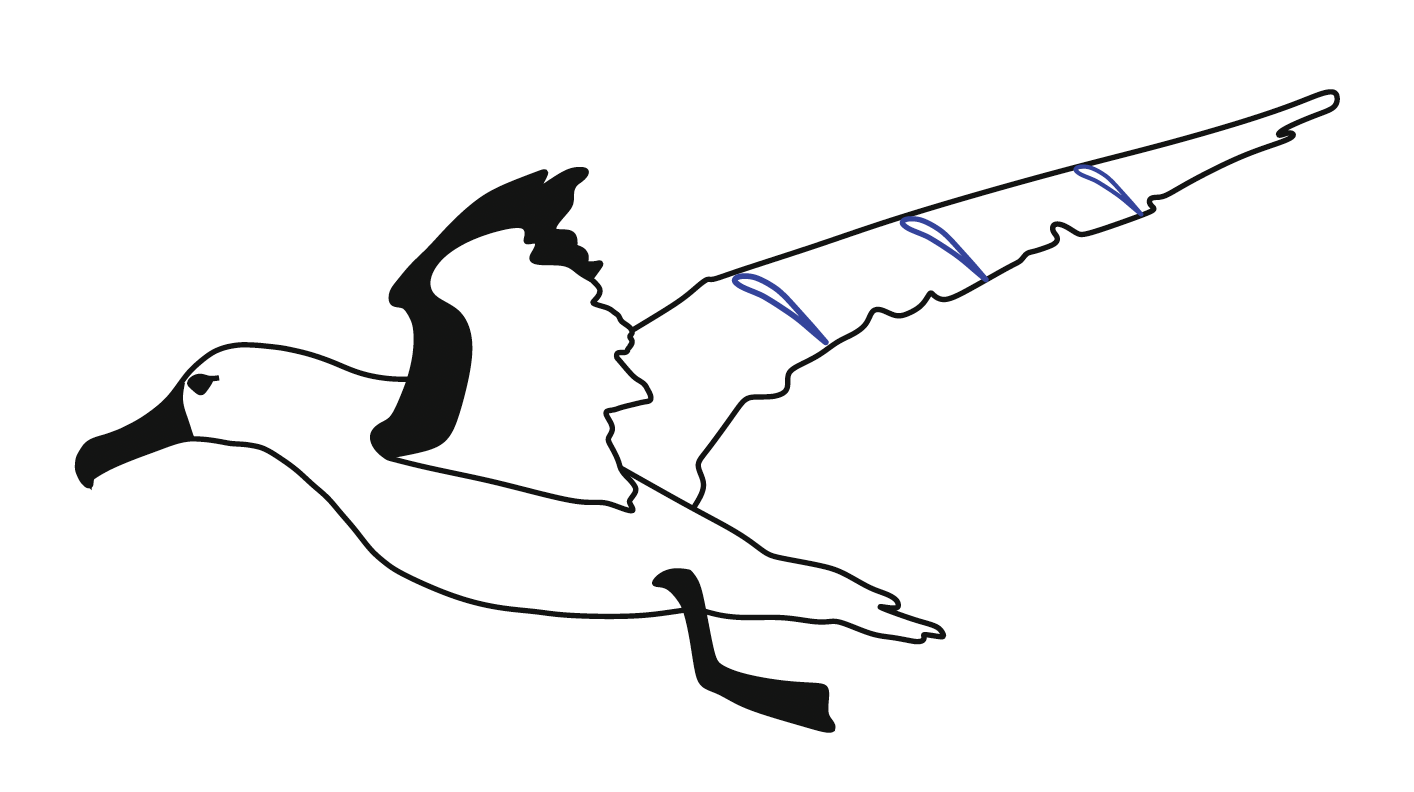
\includegraphics[width=\linewidth]{albatros.png}
\end{columns}
\end{frame}


\begin{frame}{Bio-Inspired Propulsion}
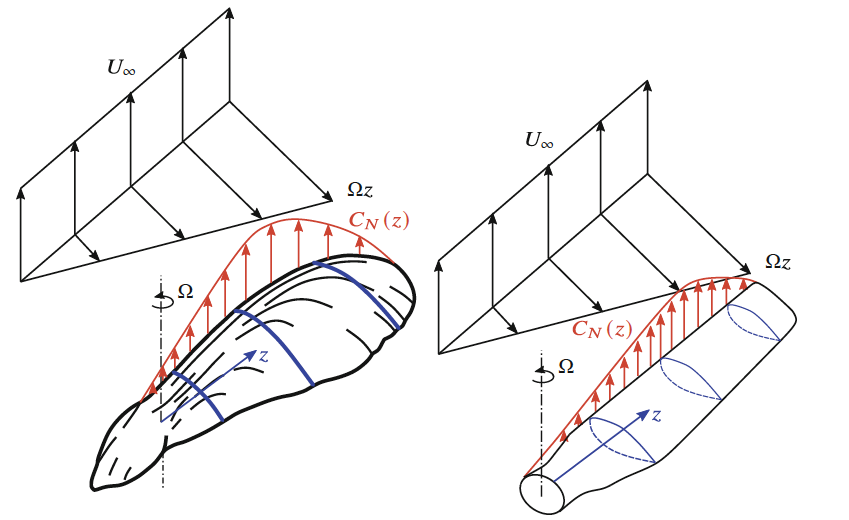
\includegraphics[width=\textwidth]{bio-prop.png}
\end{frame}

\begin{frame}{Modeling Structural Forces}
\begin{itemize}
    \item Wings split into 2D slices
    \item Forces: lift, drag, normal, axial
    \item Moments: bending (flap/edge) and torsion
\end{itemize}
\end{frame}

\begin{frame}{Force Components on a Section}
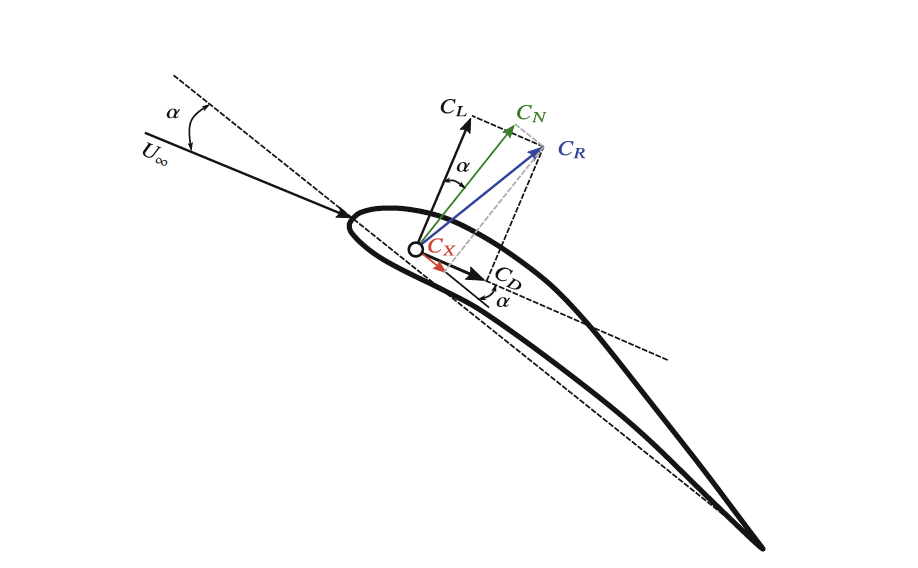
\includegraphics[width=\textwidth]{Screenshot 2025-06-30 at 19.55.47.png}
\end{frame}

\begin{frame}{Albatross Takeoff Scenario}
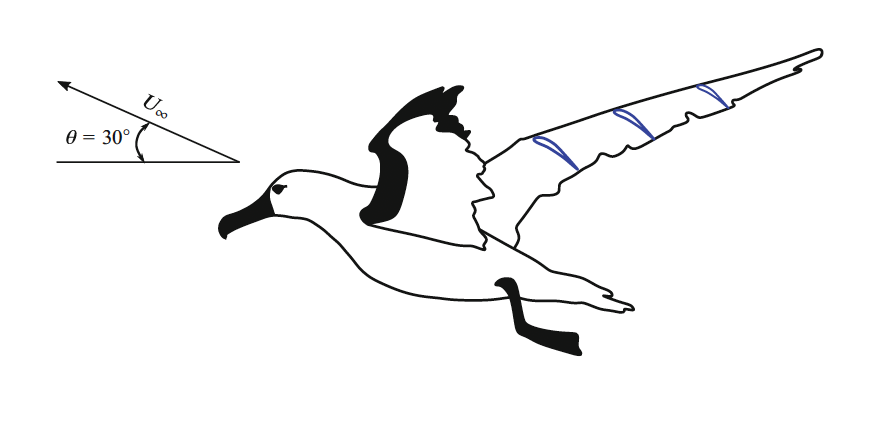
\includegraphics[width=\textwidth]{Screenshot 2025-06-30 at 19.55.43.png}
\end{frame}

\begin{frame}{Takeoff Modeling Example}
\begin{itemize}
    \item Use geometry and airspeed
    \item Apply known coefficients (C\_L, C\_D)
    \item Compute flapwise, edgewise, and torsional moments
\end{itemize}
\end{frame}

\end{document}
